\documentclass[a4paper,11pt]{article}
\pdfoutput=1 % if your are submitting a pdflatex (i.e. if you have
             % images in pdf, png or jpg format)
\usepackage{jinstpub} % for details on the use of the package, please
                     % see the JINST-author-manual

\title{REST-for-Physics, a ROOT-based framework for event oriented data analysis and combined Monte Carlo response.}

\collaboration{
\includegraphics[height=24mm]{RESTlogoFull.png}}

%% %simple case: 2 authors, same institution
%% \author{A. Uthor}
%% \author{and A. Nother Author}
%% \affiliation{Institution,\\Address, Country}

% more complex case: 4 authors, 3 institutions, 2 footnotes
\author[a,b,1]{F. Irst,\note{Corresponding author.}}
\author[c]{S. Econd,}
\author[a,2]{T. Hird\note{Also at Some University.}}
\author[c,2]{and Fourth}

% The "\note" macro will give a warning: "Ignoring empty anchor..."
% you can safely ignore it.

\affiliation[a]{One University,\\some-street, Country}
\affiliation[b]{Another University,\\different-address, Country}
\affiliation[c]{A School for Advanced Studies,\\some-location, Country}

% e-mail addresses: only for the forresponding author
\emailAdd{javier.galan@unizar.es}
\emailAdd{bur\_ning@sjtu.edu.cn}

\abstract{Abstract...}


\keywords{Software architectures (event data models, frameworks and databases);Simulation methods and programs;Data processing methods;}

%\arxivnumber{1234.56789} % only if you have one


% \collaboration{\includegraphics[height=17mm]{example-image}\\[6pt]
%   XXX collaboration}
% or
%\collaboration[c]{on behalf of XXX collaboration}

% if you write for a special issue this may be useful
%\proceeding{N$^{\text{th}}$ Workshop on X\\
%  when\\
%  where}

\begin{document}
\maketitle{}
\flushbottom
%%%%% I create sections, but it is just orientative. Some sections may disappear and get integrated in other sections. It is just to do not forget to talk about something.

\section{Introduction}
\label{sec:intro}

% Motivation for software development

% Emphasize also its academic use

% What it is?
REST-for-Physics (Rare Event Searches Toolkit for Physics) is a collaborative software effort providing a common framework and tools for acquisition, simulation, generic data analysis, and detector response in experimental particle physics. An ambitious feature of REST-for-Physics is its capability to analyze together and compare Monte Carlo and experimental data using the same \emph{event processing} routines upon a unified \emph{event data} - \emph{metadata} architecture. 

% Describe motivation. 
The framework was born to bring together different software requirements related to gaseous Time Projection Chambers (TPCs) in the context of Rare Event Searches, and to unify and coordinate various independent developments in a common modular infrastructure with potential for scalability and reusability. Special care has been taken to ensure the traceability and reproducibility of the results obtained after the data processing, linking the code version with the metadata version stored on disk, and protecting such relation. Any user local changes are identified at compilation time, and it is used to guarantee that the version executed and the results written to disk correspond to an unmodified official public release. This fact is extremely relevant when planning to register official experimental data and preserve it for historical reasons. Our code updates are periodically published at the zenodo citations system, where we find our latest official release today\,\cite{javier_galan_2021_5092550}.

% Add historical context?
REST-for-Physics is the result of several years experience on detector physics and research, motivated originally to cover the software needs of the T-REX project for neutrino and dark matter searches~\cite{Irastorza:2015dcb,Irastorza:2015geo}. The REST-for-Physics code has benefited from several academic works, as it becomes apparent in several PhD. thesis publications\,\cite{IguazThesis,tomas2013development,SeguiThesis,HerreraThesis,GraciaThesis, GarciaPascualThesis, RuizThesis}, that have contributed to shape and define the final project that we describe in this manuscript.
This project has contributed to develop different but interconnected research activities in a coherent way, unifying common tools that are used today regularly not only in research but also at all the academic levels, from undergraduate to master students. 

Different experimental projects have seen REST-for-Physics growing from its preliminary stages to the mature project we present in this work. REST-for-Physics has been evolving and it is being used to produce results at CAST~\cite{Anastassopoulos:2017ftl}, TREX-DM~\cite{trexdm_bckmodel}, PandaX-III~\cite{pandaxiii_cdr,Lin:2018mpd,Galan:2019ake}, and IAXO~\cite{Armengaud:2019uso}. In addition to sharing the know-how and experience in our physics domain, the motivation to release a public common framework resides on providing the possibility to distribute the experimental data following a unique format readable with REST-for-Physics, or any other \emph{ROOT} I/O compatible code in a future open-data program of the experiment. The code is open-source and it is distributed under a GNU public licence at \emph{GitHub}\,\cite{REST_Git}.

The aim of this document is to give the reader a broad perspective of the purpose of the software project, its organization and contents, and the basic instruments that shape the whole infrastructure, giving an idea of its scalability potential, and in addition, showing the code validation strategy and continuous integration philosophy. For further reference we provide detailed information, including an API class documentation for developers\,\cite{REST_API} daily synchronized with the latest development version, and a comprehensive guide for first time users\,\cite{REST_user_guide}. We also offer an additional communication channel in the shape of forum\,\cite{REST_forum} to encourage discussion about topics related in our domain, help others on their first steps using REST, or integrate their first routines inside the framework, and discuss about new or existing features upgrades.

% The class code documentation is compiled using \emph{Doxygen} markdown and hosted at a server at the University of Zaragoza\footnote{\url{https://sultan.unizar.es/rest}}. There is a documentation user guide available at XXX.

% Projects involved in the use and development of REST: CAST, IAXO, PandaX-III, TREX-DM.

%% Monte Carlo and experimental common processing discussion
%% This is possible by using those \emph{event processes} to condition the input data generated, for example, by a \emph{Geant4} Monte Carlo simulation. After an appropriate \emph{event data} conditioning, our Monte Carlo generated event will reproduce the \emph{rawdata} of the detector acquisition. Once we are at that stage, we can benefit from using the same \emph{event processes} to analyze Monte Carlo and real experimental data. A realistic Monte Carlo \emph{rawdata} reconstruction will allow us to assess, validate and optimize the processes that will be involved in the real event reconstruction and analysis even before the start of the physics run of the experiment.


% Results already produced by REST in the past

% Academic impact of REST-for-Physics
\section{General description}
\label{sec:framework}

% Table with useful information, code version, github address, zenodo reference, documentation

% Mention physics units, basic geometrical routines TRestPhysics, TRestMesh, ...

\emph{REST-for-Physics} is composed of a set of libraries written in C++ and it is fully integrated with ROOT~\cite{ROOT,Brun:2011Gp,ROOT2011}, i.e. most C++ classes inherit from a ROOT TObject and therefore they can be read, accessed or written using the ROOT I/O interface. The only structural dependence is related to ROOT libraries, while other packages, as \emph{Geant4}~\cite{Agostinelli:2002hh} or \emph{Garfield++}~\cite{Garfield}, can be optionally integrated and used within the \emph{REST-for-Physics} framework when generating or processing Monte Carlo data. Being \emph{REST-for-Physics} a natural extension of ROOT, we follow the same naming conventions, which are the Taligent rules. On top of those standard naming conventions, any \emph{REST-for-Physics} C++ class (object) will be always started by the \emph{TRest} prefix. In this manuscript we will highlight the words when they clearly make a reference to an existing \emph{REST-for-Physics} C++ object. I.e. an object named \emph{TRestEvent} will be written in the following as \emph{event} or an object named \emph{TRestAnalysisTree} will be written as \emph{analysis tree}. Therefore, a highlighted word, within context, expresses a deep connection with the different elements of the code.

%%%%%% THE MAIN FRAMEWORK DESCRIPTION %%%%%%%
\subsection{The REST-for-Physics framework}
Inside the \emph{REST-for-Physics} ecosystem we may distinguish a main library, or framework, that prototypes and fixes the implementation of most of the \emph{REST-for-Physics} elements. Those base objects serve to define common methods and data members for specific\footnote{The reader should notice that when we refer to specific objects, we refer to objects which inherit, in the strict sense of C++ object inheritance, from the base abstract objects, \emph{event}, \emph{metadata} and \emph{event process}. In the text, we will highlight the keyword \emph{specific} to refer to those inherited objects in a generic way, i.e. \emph{specific event} will be connected to any \emph{TRestSpecificEvent} or \emph{specific event process} would be connected to any \emph{TRestSpecificProcess}. It is worth to notice that event and process objects contain the \emph{event} and \emph{process} keywords in their class name, while metadata classes usually omit the use of the \emph{metadata} keyword. } objects. We shall briefly introduce those basic elements.

%We briefly introduce those relevant objects, encoded as pure C++ abstract classes, and defined in the \emph{REST-for-Physics} framework.

\begin{itemize}
    \item The \emph{event} object encapsulates any specific \emph{event} data inside \emph{REST}. It defines common fields, such as timestamp or event id, and it prototypes common methods used for printing or drawing event information. A particular \emph{specific event} implementation defines a type, thus in what follows we will distinguish between the \emph{event} data as the explicit contents of a particular \emph{specific event}, and the \emph{event} type as the format, or structure, of the \emph{specific event}.
    
    \item A \emph{metadata} object can be initialized through a configuration file (at present we adopted the XML format). A \emph{metadata} class might be used as a mere information container, storing relevant parameters, that can be initialized through XML, such as the conditions of a \emph{Geant4} simulation, i.e. the \emph{geant4} metadata object, or it might adopt the shape of a complex object definition that implements advanced methods, such as the implementation of a \emph{detector readout}, or a \emph{magnetic field} volume including interpolation routines. Those advanced \emph{metadata} objects will be found at specialized libraries, some of them being detailed later on in section\,\ref{sec:libraries}. Conceptually we understand by \emph{metadata} any information required to give meaning to any \emph{specific event} data. Therefore, any input or output parameters, required during the processing or transformation of \emph{event} data, or type, using \emph{event processes}, is regarded also as \emph{metadata}. 
    
    \item The \emph{event process} object defines an input/output \emph{event} scheme allowing to interconnect different \emph{specific event process} implementations into a sequential processing chain. The \emph{event process} inherits itself from the \emph{metadata} object, since a process usually requires initialization to define few input parameters that control the behaviour of the process.
\end{itemize}

We will find other basic or elemental tools inside the main framework, such as output string helper methods, fundamental physics constants and units system, or other basic mathematical tools helping to the development of any specific \emph{event process}. Any \emph{metadata} or \emph{event process} object that does not require specific specialization will be likely hosted inside the framework domain.
 On top of that, the framework repository\,\cite{REST_Framework_Git} serves to centralize other \emph{REST-for-Physics} components, such as libraries or packages. Those components will be introduced later in section\,\ref{sec:libraries}.%SUB-MODULES

% Describe sub-modules, libraries and packages.

% framework core, tools, analysis

% define \emph{metadata} to TRestMetadata naming convention

% Submodules, Libraries, packages, projects

%%%%%% I/O Access and storage %%%%%%%
\subsection{I/O access and metadata storage}

%% Paragraph dedicated to REST progress and philosophy % Description of metadata+data concept
%% During the last years, major upgrades took place on the REST core libraries\,\cite{Galan_8thTPC}. 


% TRestRun (any event data processing taking place with REST will write to disk a TRestRun object, any REST object taking active part on the data processing will be stored in ROOT file.
\emph{REST-for-Physics} uses the ROOT I/O interface to write \emph{event} and \emph{metadata} objects to disk. A ROOT file generated with \emph{REST} may contain any number of \emph{specific event} and \emph{specific metadata} objects, including any \emph{specific event process} (being a \emph{metadata} object itself). Those objects are stored in a unique file, together with the \emph{run} metadata object and the \emph{analysis tree} that are always present at any file that has been processed with \emph{REST}. The \emph{run} object registers few important values to identify the data file, such as the start time, duration, run number, etc, while the \emph{analysis tree} collects information, named observables, at any stage of the data processing. The \emph{run} object takes also an active role when accessing the different objects stored on disk by implementing helper methods to access the data, such as getting a list of events fulfilling particular conditions at the \emph{analysis tree} or retrieving directly the pointer to a given event id number, and updating simultaneously its corresponding \emph{analysis tree} entry.

% something about metadata
% For each aspect of \emph{metadata}, we define a class with proper data members to describe it, known as \emph{metadata} structures. 
The framework philosophy is to create \emph{specific metadata} objects with dedicated data members to store any information crucial for the final analysis, and/or to fully determine the nature of the data we are storing. All the \emph{metadata} inherited objects gain data member reflection support, thus creating a relation between the C++ conceptual class members and the text fields used in our configuration files. Through the implementation of the \emph{metadata} object we have designed a dedicated file format for \emph{REST}, based on Extensible Markup Language (XML). This upgrade allows us to read XML files with additional features, such as using system environment variables, complex programming instructions, including \emph{if} conditions or \emph{loops}, evaluation of mathematical expressions, or support for arbitrary physical units conversion inside any parameter.

Using the \emph{metadata} philosophy we create a unique relation between the configuration files and the C++ objects. One XML element is identified with one \emph{metadata} object, with its attributes associated to the data members inside the object. If there is an embedded element inside the XML element, it is associated in-chain to a \emph{metadata} data member of the \emph{metadata} object. In this way, the automatic initialization of \emph{metadata} objects is achieved, without any file reading methods in the class.

%% RML --> system environment variables + loops + mathematical expression evaluation + physical units support in parameters



%% SHALL WE ILUSTRATE THIS WITH SOME CODE? Such as Int\_t fMetadataMember = 0;   is connected with `<parameter name="metadataMember" value="10"/>? 


% A link is therefore established between class data members and text fields, enabling automatic reading of configuration files. We invented a file format for REST, \emph{rml}, based on Extensible Markup Language(xml). We believe the strong hierarchy and attribute sets provided by xml are beneficial in our application. All the running jobs, such as simulation, analysis, and file generation, are based on \emph{rml} encoded configuration file. 

%% metadatda and rml. Shall we explain rml?
% rml --> metadata class's data members. We now set a convention for rml parameters linked to metadata class's data members. **configurability** could be explained on "reflectable metadata"


%%%% This paragraph will be considered at detector library, and at data processing chain.
%% In addition to the storage of value sets, we have various tool methods provided by the \emph{metadata} structures which is useful in the analysis. For example in detector readout topology we enable readout channel position finding according to the daq ID, and in gas property we can calculate electron drift speed with certain external libraries.Any created \emph{metadata} structures will be stored to the output file. Moreover, any previous existing \emph{metadata} structures from input file will be transferred to output file. Traceability and reproducibility of REST data would be enhanced with this file logic. 

% something about event data
%% Basic introduction of data types and processes
% An event type defines a particular structure that helps organizing different entities that keep a similar relation.
%%% Multiple event types(data structures) are also defined in REST to store \emph{event data}, which could be generated either in data acquisition, simulation or data processing. The inherited common data fields, such as event id, time, tag, keeps continuity of data flow, while the special fields contained in each types conduct best structured data for different stages of analysis. Common interfaces are also implemented for visualizing and printing the \emph{event data} for each type of event. In addition, we also implemented various tool methods associated to the nature of each data structure, for example points rotation, Fast Fourier Transform (FFT), which helps to develop analysis code quickly. Each type of \emph{event data} is stored in an individual branch in the tree in the output file, helping to check the condition of each stage of analysis.

\subsection{Event data processing and analysis}

The framework allows us to build an event data processing chain in a modular way by interconnecting already existing \emph{specific event processes}, or to develop new ones with the potential to plug it directly to an existing processing chain. Each \emph{event process} has access to the input \emph{specific event}, the \emph{analysis tree}, and any \emph{metadata} object that it is accessible by the \emph{run} object. Depending on the input/output \emph{especific event} interaction inside the process we may attempt to classify the \emph{event processes} into four different groups.

\begin{itemize}
\item An \emph{external process} is a process that reads an external data source usually at the beginning of a \emph{REST} processing chain. It might be binary data generated by an acquisition system, or Monte Carlo data generated by an external simulation package. The process will be in charge of understanding the format of that external data and translate it into a \emph{REST specific event}.

\item An \emph{internal process} is a process in which the \emph{specific event} input is the same type as the \emph{specific event} output. Most of the processes are in this kind, and are placed inside different libraries according to their aspects of data analysis. If an \emph{internal process} does not change the \emph{event} data, i.e., reads only \emph{event} data and produces observables, it is also called \emph{pure analysis process}. 

% pure analysis process was mixing with general process

\item A \emph{transformation process} is a process that receives as input a \emph{specific event} and transforms it to a different \emph{event} type. This kind of processes will be all placed at the \emph{connectors} library, described on section\,\ref{sec:libraries}, in order to encapsulate all library inter-dependencies at a single entity. 

\item A \emph{general process} is a process that does not need a \emph{specific event} type as input. In other words, it does not need to read \emph{event} data. It may take information from the \emph{analysis tree} to draw figures and save to png file, or read system information to store directly as observables. This kind of process will be likely placed at the main framework, since no physical jobs are contained.
\end{itemize}



% Event transformation
A \emph{specific event} might be transformed during the event processing and, in that transformation, relevant information might not be available anymore at the final transformed output event. The reason is that the role of the \emph{specific event} object is to provide a faithful or significant representation of the data at the state of processing where we are inside our processing chain, i.e. at different processing stages we might have the event data made of time signals registered at an electronics setup, or we might have the event data in the shape of discrete energy deposits at a physical coordinate system. Therefore, the transformation from one event data representation, or \emph{specific event}, into another, carries as a consequence that a relevant parameter available at a particular stage, is not available anymore (or it is harder, less intuitive, accessing to it). 

% Analysis tree description
The \emph{analysis tree} comes into play as an instrument to collect all those parameters extracted or calculated from the \emph{specific event} information and that will be relevant for the final analysis.  Any \emph{specific event process} in the processing chain is allowed to add new observables to the \emph{analysis tree}. Once a process adds an observable to the \emph{analysis tree} this observable will be always available even if the \emph{event} data is transformed or the processing chain happens in several steps using different input/output \emph{REST} data files. The information at the \emph{analysis tree} is always accumulative, and therefore it will contain a full summary of the observables added by each process.
%, following the decisions taken by the person in charge of the data chain design. 
In brief, the \emph{analysis tree} provides a way for \emph{specific event processes} to export an analysis result to the framework.

The information extracted by a process and added to the \emph{analysis tree} might be as simple as just a registered value from the \emph{specific event} at a given stage of the processing chain, or it might be the result of a complex calculation in the context of a physics model, including complicated input \emph{metadata} objects or parameters. Of course, even in the case of basic observables extracted directly from the \emph{specific event}, the user might be interested to know the evolution of such observable after an intermediate processing. In order to do that, it is possible to define the same \emph{specific event process} twice at different positions in the sequential processing chain.


%defines a particular analysis job upon a particular input event in order to manipulate the \emph{specific event} data, transform it and extract relevant information. 

%Afterwards the \emph{event process} must yield an output event. 

%In principle, any \emph{event process} that participates in a data processing chain must satisfy that its input event type corresponds with the output event type of the previous \emph{event process}. 

The \emph{event process} object implements a method to facilitate the addition of observables to the \emph{analysis tree}. This method allows to create automatically a new observable from any C++ variable (including various C++ types, from base types to proper \emph{stl} containers). We do not need to care about global values and their addresses by using this method. Weakening the concept of a ROOT TBranch and TTree helps us to reduce the number of lines in the code, while focusing more on analysis.

%% discuss how to analyze Monte Carlo and experimental data using common event processes
Our framework design is completely transparent to the processing of real experimental data, or Monte Carlo simulated data. The reason is that a \emph{specific event process} implementation may operate on both scenarios. The only requirement is that the experimental or simulated input \emph{event} must be given to the process in the form of a \emph{specific event} type. If both, simulation or experimental data, are conditioned to fit in a common \emph{specific event} type, we will be able to build a processing chain that not only processes simulated data or experimental data, but that fully combines both. As a hypothetical case, we could integrate a process simulating the signal shaping of electronics into real experimental data to assess the benefit of applying such electronics setup in our real experiment. Furthermore, a proper conditioning of the generated Monte Carlo \emph{event} data will allow us to evaluate the algorithms for analysis to be used with the real experimental data even before the start of the physics data taking program.

%Either Monte Carlo or experimental data can be the input of \emph{event processes}. 
% For the Monte Carlo data, with properly conditioned simulation \emph{event processes}, we can reproduce the raw data of the detector acquisition. Once at that stage, by reusing common \emph{event processes}, we can analyze the simulation data just as experimental data. Algorithms can be developed with optimized data selection efficiency even before 


% Discuss the analysis tree(what's better than basic tree) and idea of observable
%REST provides an uniformed target, \emph{observable}, for the \emph{event processes} to export analysis result. 
%\emph{Observable} is defined as any information extracted from \emph{event data}. 
%It could be the raise times of each pulses in an event, the reconstructed event vertex/energy, the background likelihood of the event, etc. 
%Multiple \emph{observables} can be associated to the \emph{event data}, forming a list of event properties. 


%% discussion about multi thread 
Event processes are executed through an efficient engine with multi-thread support. The data processing chain is cloned into multiple instances and kept in different threads respectively. During execution, the input event is in turn dispatched to each thread for processing, while the output event is redirected to the global output file for writing, leading to an increase of processing speed proportional to the number of threads enabled. Figure\,\ref{fig:processing} summarizes the input/output processing logic and the different concepts previously described in this section.   %Multi-thread operation is most helpful in case of algorithm verification, for example we can quickly get the result of a newly added observable to see if the code is alright.

\begin{figure}[htb!]
  \centering
  \raisebox{-0.5\height}{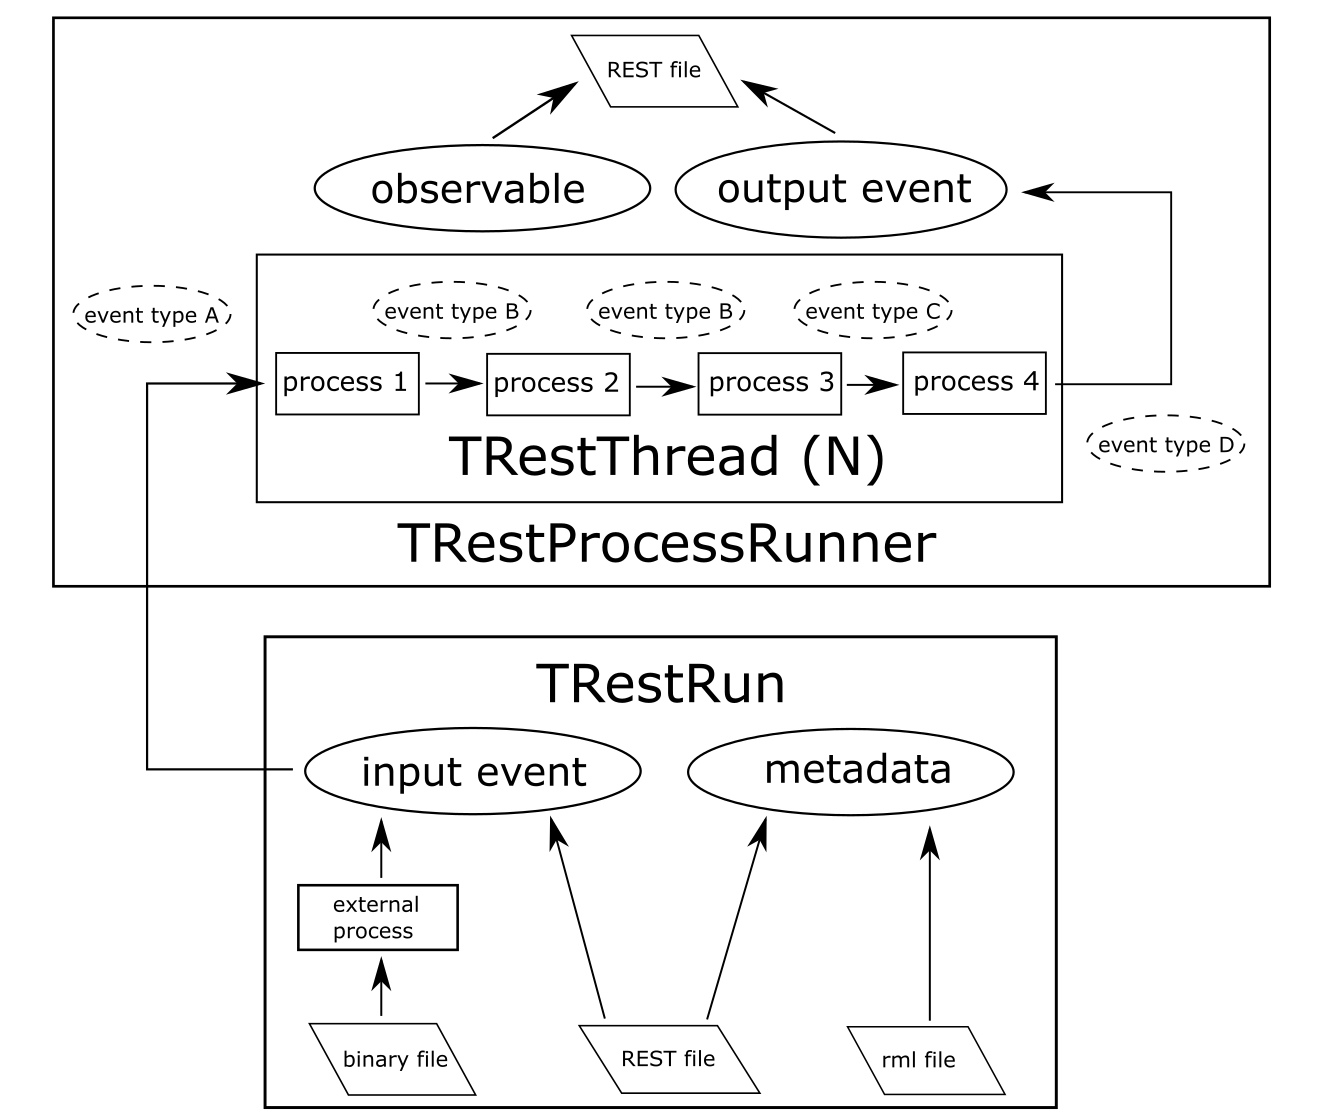
\includegraphics[width=0.75\linewidth]{images/process_chain.png}}
	\caption{A schematic showing the event data flow inside a \emph{REST} processing chain. The \emph{run} object is initialized, and it has access to any \emph{specific metadata} or \emph{event} data available at the input \emph{REST} file, or any additional objects described through \emph{rml}. The data is then processed using the implementation inside the \emph{process runner} object. Different event types (A,B,C,D) make reference to different \emph{specific event} implementations. The resulting output \emph{REST} file will contain all the \emph{metadata} information available to the chain, including any previously available, together with the transformed output \emph{specific event}, and the updated \emph{analysis tree}.  }\label{fig:processing}
\end{figure}


% Define different event processing types: pure analysis.

% - Specific analysis process. It needs to access a particular event data type (it will be placed then at the corresponding library defining that event type).
% - Pure analysis process. It only requires access to the analysis tree (and therefore it will be placed at the main framework).
% - Conversion process. It is a process that interconnects 2 libraries by transferring an event type into another. Therefore, this kind of process will be placed at the dedicated `connectors` library.
% We usually write \emph{event processes} in two major ways, identified by whether transforming the type of \emph{event data}. If the output event is transformed into another type, it is a \emph{conversion process}. If it operates in a particular event type, i.e. \emph{hit}, \emph{raw signal} or \emph{track processes}, in which the output event type remains unchanged, it is an \emph{analysis process}. In the following sub-sections we provide a description of the different processes involved in our data processing. A full, detailed and up-to-date list of documented processes will be available at~\cite{RESTsultan} for further reference.

\subsection{Visualization and plotting}

% TRestBrowser --> event by event **visualization**
% TRestAnalysisPlot --> data statistics plot, histo
% TRestMetadataPlot --> for metadata

\emph{REST-for-Physics} implements routines for event visualization and observable plotting based on ROOT drawing objects and methods. We use ROOT graphical interface objects to create basic tools, such as an \emph{event browser} with a control panel and a drawing pad (see Figure\,\ref{fig:eventBrowser}). The drawing pad itself is the target of the \emph{draw event} method implemented at each \emph{specific event}. If enabled, different output \emph{specific event} trees - from different stages at the data processing - will have been stored in the same file. In that case the \emph{event browser} will be able to switch between the different event data representations.

\begin{figure}[htb!]
  \centering
  \raisebox{-0.5\height}{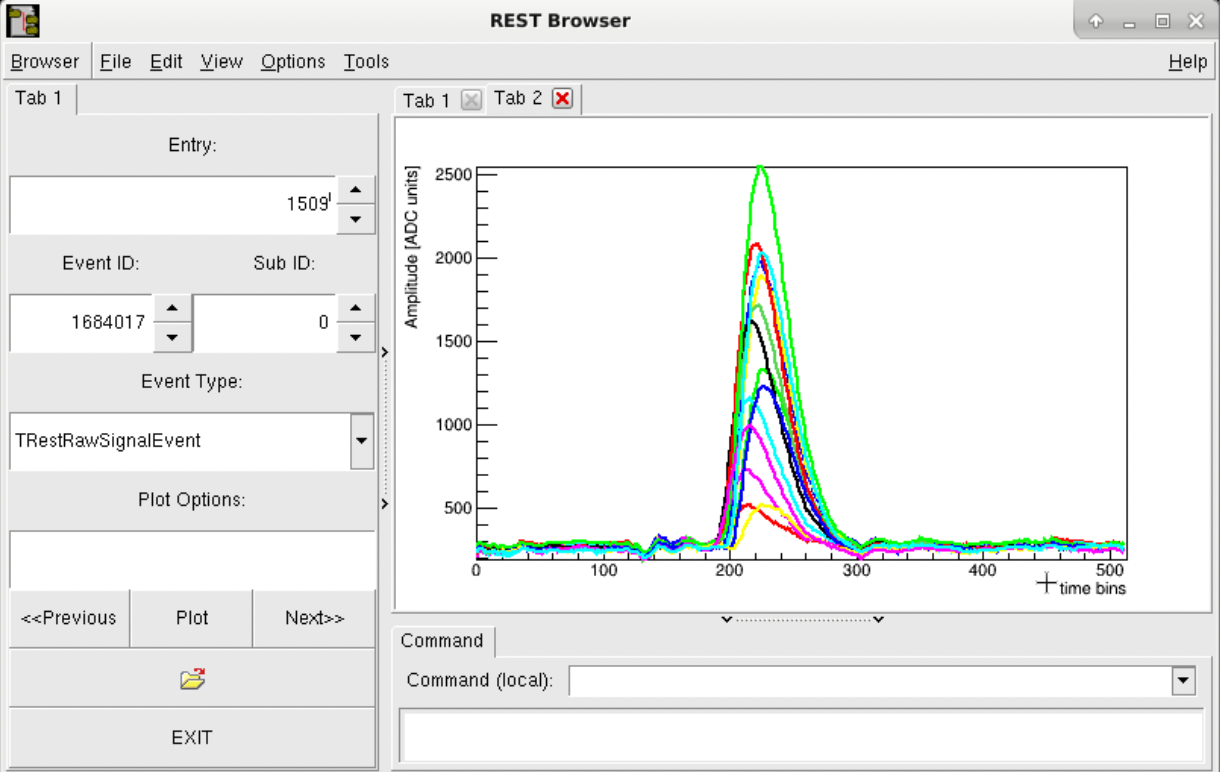
\includegraphics[width=0.45\linewidth]{images/EventBrowser.png}\,\,\,\,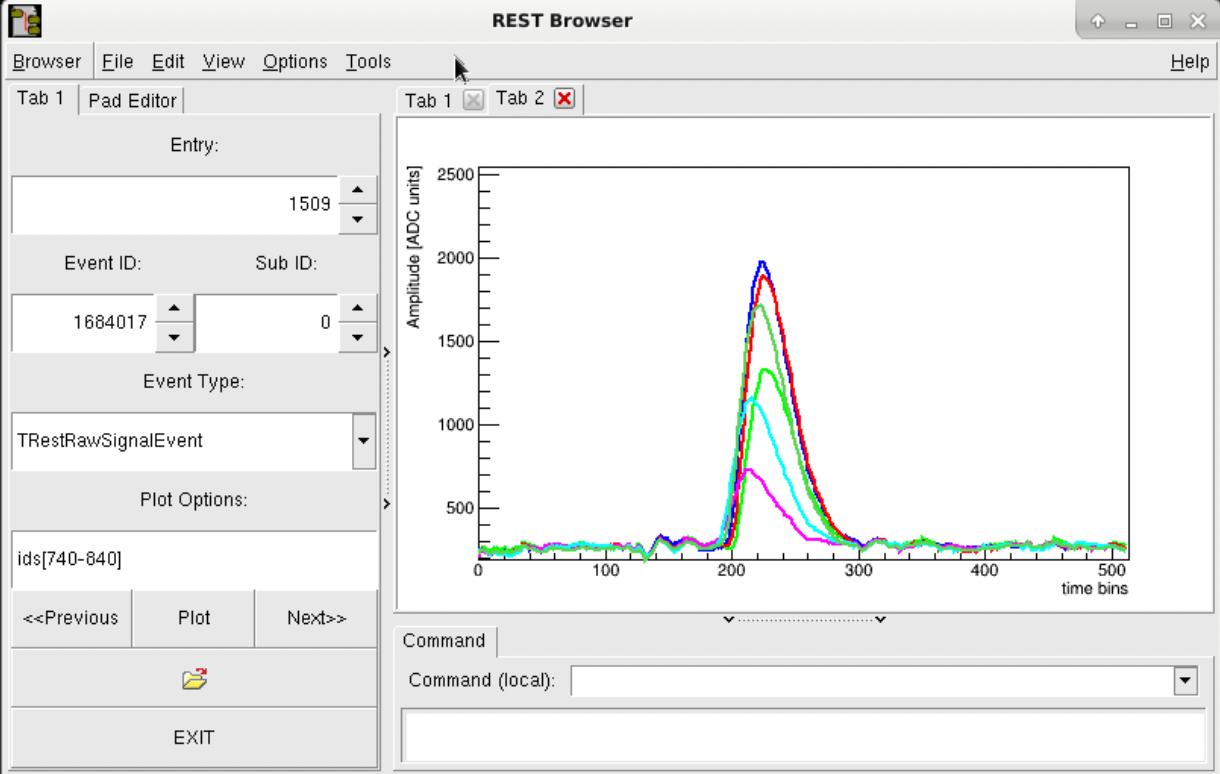
\includegraphics[width=0.45\linewidth]{images/EventBrowserSelection.png}}
	\caption{Two snapshots from the \emph{REST event browser} where we observe the control panel and the drawing pad showing an event entry for a \emph{raw signal event} (see section\,\ref{sec:libraries} for details on the \emph{specific event} type). On the left figure we present the complete event, while on the right figure the pulses have been filtered using an option passed to \emph{draw event} method implemented at each \emph{specific event}.}\label{fig:eventBrowser}
\end{figure}

%%%%%%%%%%%%%%%%%%%%%%%%%%%%%%%%%%%%%%%%%%%%%%%%%%%%%%%%%%%%%%%%%%%%%%%
%% This is true, we have the choice to put all them together. But it would be good to implement a kind of "smart" event browser that would open all the previous files used on the processing and contain event data. Then we would create a new TAB for each type on the window PAD, there where it says "TAB 1", "TAB 2".
%%%%%%%%%%%%%%%%%%%%%%%%%%%%%%%%%%%%%%%%%%%%%%%%%%%%%%%%%%%%%%%%%%%%%%%
%% THIS IS AN OPTION
%As described above, multiple event branches are stored in REST output file corresponding to the different stages of data processing. Each type of \emph{event data} contains a default visualization method to be drawn on the pad. When opening the file for visualization, one can simply switch between the entries, and view the \emph{event data} at different stages.
%%%%%%%%%%%%%%%%%%%%%%%%%%%%%%%%%%%%%%%%%%%%%%%%%%%%%%%%%%%%%%%%%%%%%%%

The \emph{analysis tree} object inherits directly from a ROOT TTree object, and therefore we may exploit all the resources provided by ROOT when analysing the observables that have been added to the \emph{analysis tree} by the different \emph{specific event processes} at the processing chain. I.e. we can use a ROOT TBrowser to explore the \emph{REST} data files, and quickly draw and inspect few variables from the \emph{analysis tree}. 

Furthermore, \emph{REST} implements dedicated tools for automatic and systematic plot generation, such as the \emph{analysis plot} or the \emph{metadata plot} objects. 
The \emph{analysis plot} will efficiently integrate the capability to merge thousands of files through a \emph{rml} file where we will define the plots that we want to produce with the combined data, including few advanced features such as classifying the produced histograms as a function of any \emph{specific metadata} member stored in the files, or define cuts based on the \emph{analysis tree} observables that serve to filter the data to be plotted. The \emph{analysis plot} object allows us to create a plot definition that can be used, for example, to produce quick analysis reports in \emph{pdf} format or to export histogram data in any other file format supported by ROOT.
The \emph{metadata plot} object will allow us to read many \emph{REST} generated files and draw any \emph{specific metadata} member as a function of another \emph{specific metadata} member extracted from each of the \emph{REST} files provided. This will allow us to study for a long data-set the correlation between any two metadata parameters, or to plot the evolution of a metadata parameter as a function of the \emph{run} start time, or the associated run number, for example.

%Histograms of \emph{observables} are generated with REST's analysis plot logic. Pads, plots, axis, legends, or even sub-pads and sub-plots, can all be defined through our \emph{rml} configuration file, ensuring better hierarchy and readability than C++ codes. Multiple files can be merged to a single figure or be classified into different figures. Figures can be drawn into pdf files with a single command. 

% TRestAnalysisPlot, TRestMetadataPlot, ...

\subsection{Execution and job management}
% restRoot, macros, practical data chain processing definition
Two executables are provided on the top level of the \emph{REST-for-Physics} framework and are always available to any \emph{REST} user, \emph{restRoot} and \emph{restManager}. 
\emph{restRoot} provides a ROOT interactive prompt with \emph{REST} libraries loaded, and optionally, with all the available \emph{REST} macros preloaded. 
\emph{restManager} manages the execution of jobs. It might launch a processing chain defined through the \emph{process runner}, execute a method defined at any \emph{REST} object available to the \emph{run} object, or launch a ROOT C++ macro file. On top of that, macros might have been assigned an alias to allow the system to launch macros execution through \emph{restManager} with a single command. Packages, or applications, that link to \emph{REST} libraries will also provide their own executables, such as \emph{restG4} or \emph{restFileIndexer}  (see Figure~\ref{fig:executables}). \emph{restManager} allows to define all those actions through a configurable \emph{rml} file, but on top of that, the \emph{manager}, executed through the \emph{restManager} executable, guarantees that the event data processing flow follows the standards previously described in Figure~\ref{fig:processing}.

\begin{figure}[htb!]
  \centering
  \raisebox{-0.5\height}{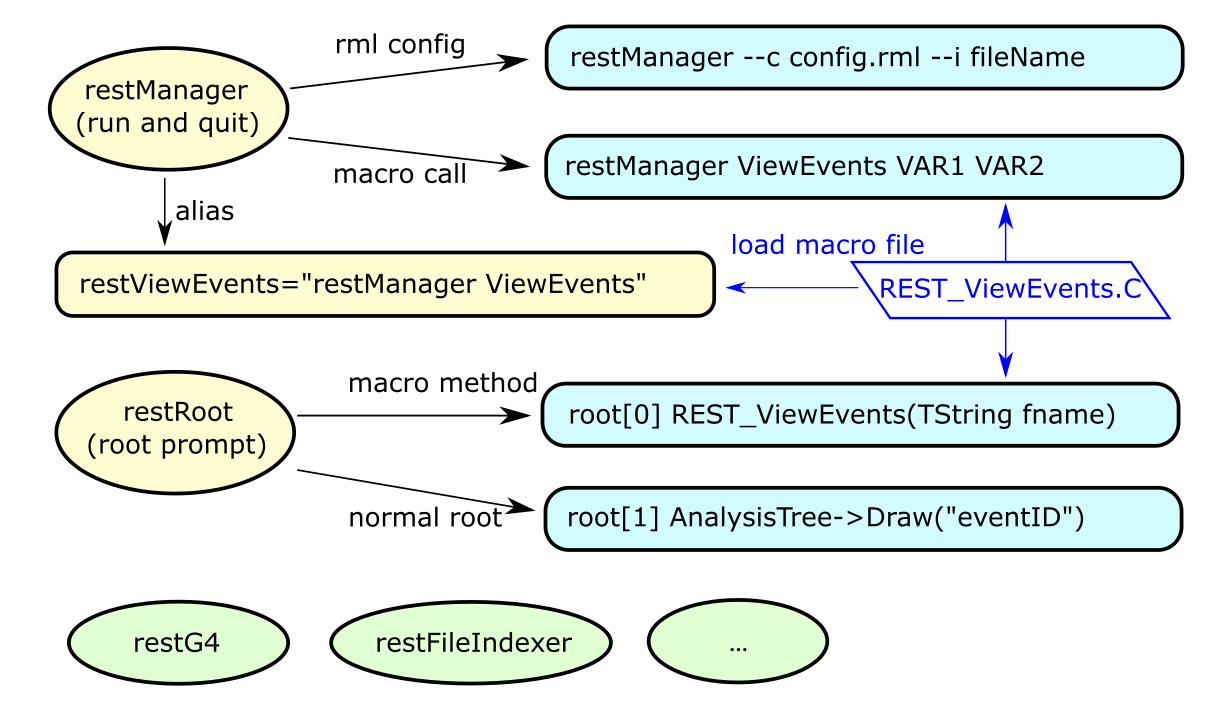
\includegraphics[width=0.9\linewidth]{images/executables.png}}
	\caption{REST executables running logic. \emph{restManager} and \emph{restRoot} work together to provide full access to the REST framework functionalities. Pre-defined ROOT C++ macro files are accessible through different interfaces, as it is shown through the \emph{REST\_ViewEvents.C} macro. Applications based on REST framework (green bubbles) extend the scope of the framework by providing additional functionalities, such as \emph{restG4} or \emph{restFileIndexer}.}
	\label{fig:executables}
\end{figure}

On top of that, a bash script, \emph{rest-config}, is generated at each project compilation to provide information on the configuration of a particular build and to facilitate the linking of \emph{REST} with external applications. 

\subsection{Project structure, versioning and code validation}
% submodule strategy

The main framework defines the basic functions, and describes the behavior of the main elements of \emph{REST}. As previously mentioned, it also serves to centralize all the \emph{REST-for-Physics} components, such as packages or libraries, and eventually dedicated projects. We have adopted a \emph{git submodule}\footnote{From this point we introduce few concepts connected with the code versioning system, \emph{git}, that are broadly available online, such as \emph{commit} or \emph{submodule}. When we refer to those alien concepts we will highlight it using the \emph{git} keyword followed by the specific concept name.} strategy to integrate those components in a modular way inside the main framework repository. This scheme allows us to independently monitor the development activity at each of those components, to isolate technical issues, and to focus on their functionality. Each component evolves independently with its own version or tracking system. A particular state of the code at each of those components is fixed at the main framework through a \emph{git commit} hash, or unique number. When that happens we say that the corresponding \emph{git commit} becomes the official component version of \emph{REST}.

The framework repository fully centralizes the versioning system of \emph{REST}, understood as the state of the code at a given period of time, including the state of the official \emph{submodules} attached to it. Any \emph{REST metadata} object written to disk using the ROOT I/O scheme will be stamped with metadata values that assure that the data written to disk has been processed with a given version, or state of the code. In order to certify that, two of those metadata members will be initialized at the code compilation time. The first metadata member will assure the source code was built from a clean unmodified state respect to the \emph{git remote} repository, and the second metadata member will certify that the corresponding framework code state is associated with an official \emph{git tag} release, where each \emph{git tag} generated at the main framework repository will automatically produce a code release referenced and citable at the \emph{Zenodo} system\,\cite{javier_galan_2021_4692983}.

On top of that versioning strategy, it is important to mention that \emph{REST} properly implements the ROOT schema evolution and assures backwards compatibility for objects that have suffered changes on their data members.

%Those libraries and packages are kept as \emph{git submodules} of REST main framework, with their versions evolving independently. Therefore, the development of \emph{sub-modules} could be separated from the main framework, contributing to a series of git repositories under multi-person work. During installation, specific libraries for different workloads can be selected to download, compile and install.

% no need to explain TRestTask since it doesn't bring new concept

% \subsection{Basic tools}
% versioning strategy
% pipeline  validation

To ensure the code quality and stability with time, each repository integrates a validation pipeline where basic tests on the code are performed, such as code formatting and style validation, testing the proper libraries integration and building of executable programs or, even more important, testing basic results from complex data processing chains (see Figure\,\ref{fig:pipelines}). Each modification to the code, or \emph{commit}, will be verified by running those validation pipelines. If a modification to the code produces an unexpected value on a consolidated data processing routine, the contributor will be notified, and changes will only become official after peer review of the code. This fact is extremely relevant to guarantee that our algorithms keep producing the expected results, or in the undesired case of a bug code identification, promptly identify the affected routines after bug correction. On top of that, validation pipelines might serve as running examples to show the integration or use of a specific tool or element operating inside the framework.


% \subsection{Pipeline validation.}

\begin{figure}[htb!]
  \centering
  \raisebox{-0.5\height}{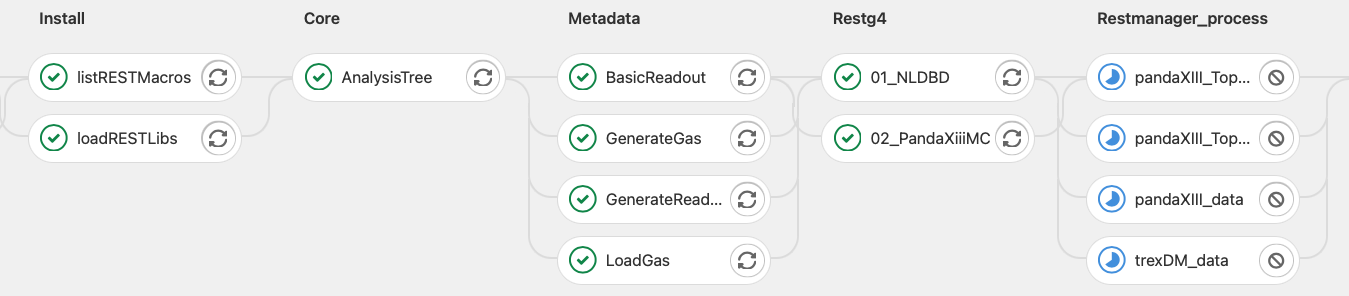
\includegraphics[width=0.75\linewidth]{images/pipelines.png}}
	\caption{A snapshot from a validation pipeline at \emph{gitlab.cern.ch} running different tests triggered by an update to the code at the main framework repository. We observe different validation stages, from the most basic tests on the left, including compilation and installation to complex data chain processing tests on the right.}\label{fig:pipelines}
\end{figure}


%section{Code structure and data traceability.}
%\input{03_structure}

% Libries and packages could be merged into one?
\section{REST-for-Physics libraries}

\label{sec:libraries}
% We define the different libraries in REST with a short description. We dedicate a section to the detector library since it is a central library that connects raw, geant4, and track libraries. And since REST was born to be used in the domain of rare event physics we always need a detector, but we are not forced to use it.

The main framework contains common tools required for centralized data access, visualization, and basic analysis routines, including generic \emph{REST-for-Physics} \emph{metadata} objects and \emph{processes} that do not require \emph{event} specialization, i.e. they only need to access information at the \emph{analysis tree} level. More specialized routines, requiring a dedicated \emph{event} data type, such as time signal processing or detector event reconstruction, are organized into libraries where all objects belonging to the library keep a closer relation and therefore enhanced connectivity. 

A library is usually associated only to one or two \emph{event} data types, improving the connectivity between different \emph{processes} inside the same library. This allows that processes "living" inside a particular library can be connected at any order and combination, as defined by the user. A dedicated library, the \emph{connectors} library, hosts those \emph{processes} or \emph{metadata} objects that need to interconnect different libraries, keeping all inter-library dependencies bounded together into a single entity, and allowing each library to be fully operational in stand-alone mode. New libraries might be added in the future to the framework, here we briefly describe those fundamental libraries that gave \emph{REST-for-Physics} enough functionality and versatility to be used in different aspects of rare event searches experiments.

\subsection{The detector library}

The detector library\footnote{\url{https://github.com/rest-for-physics/detectorlib}} is mainly used for event reconstruction inside a Time Projection Chamber (TPC). This library contains metadata objects that allow to describe the detector configuration and properties, such as the gas   in to define a detector readout topology, and access gas or other detector properties. It also implements processes including routines for event reconstruction from real detector data, and/or emulation of different physical response effects, such as electron diffusion.

\begin{figure}[hb!]
  \centering
  \raisebox{-0.5\height}{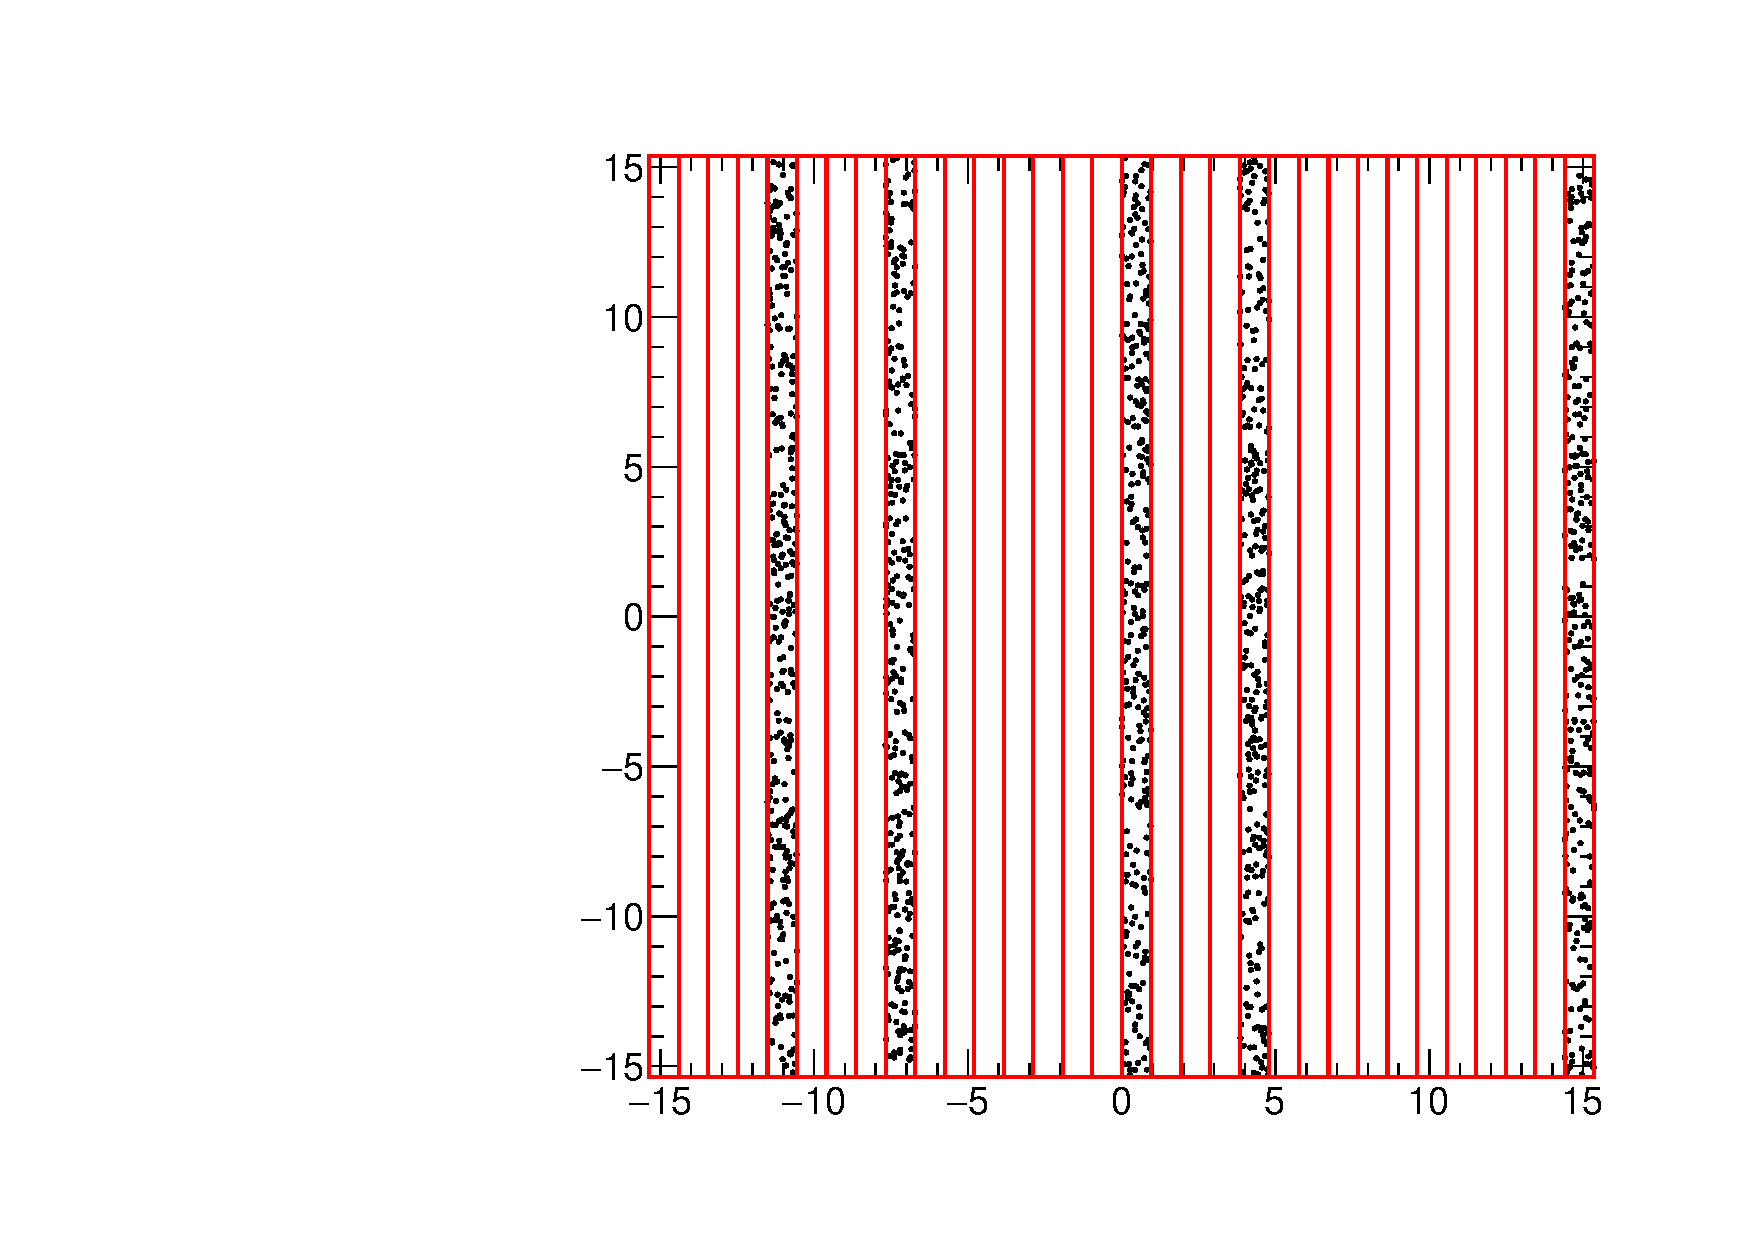
\includegraphics[width=0.3\linewidth]{images/stripped.pdf}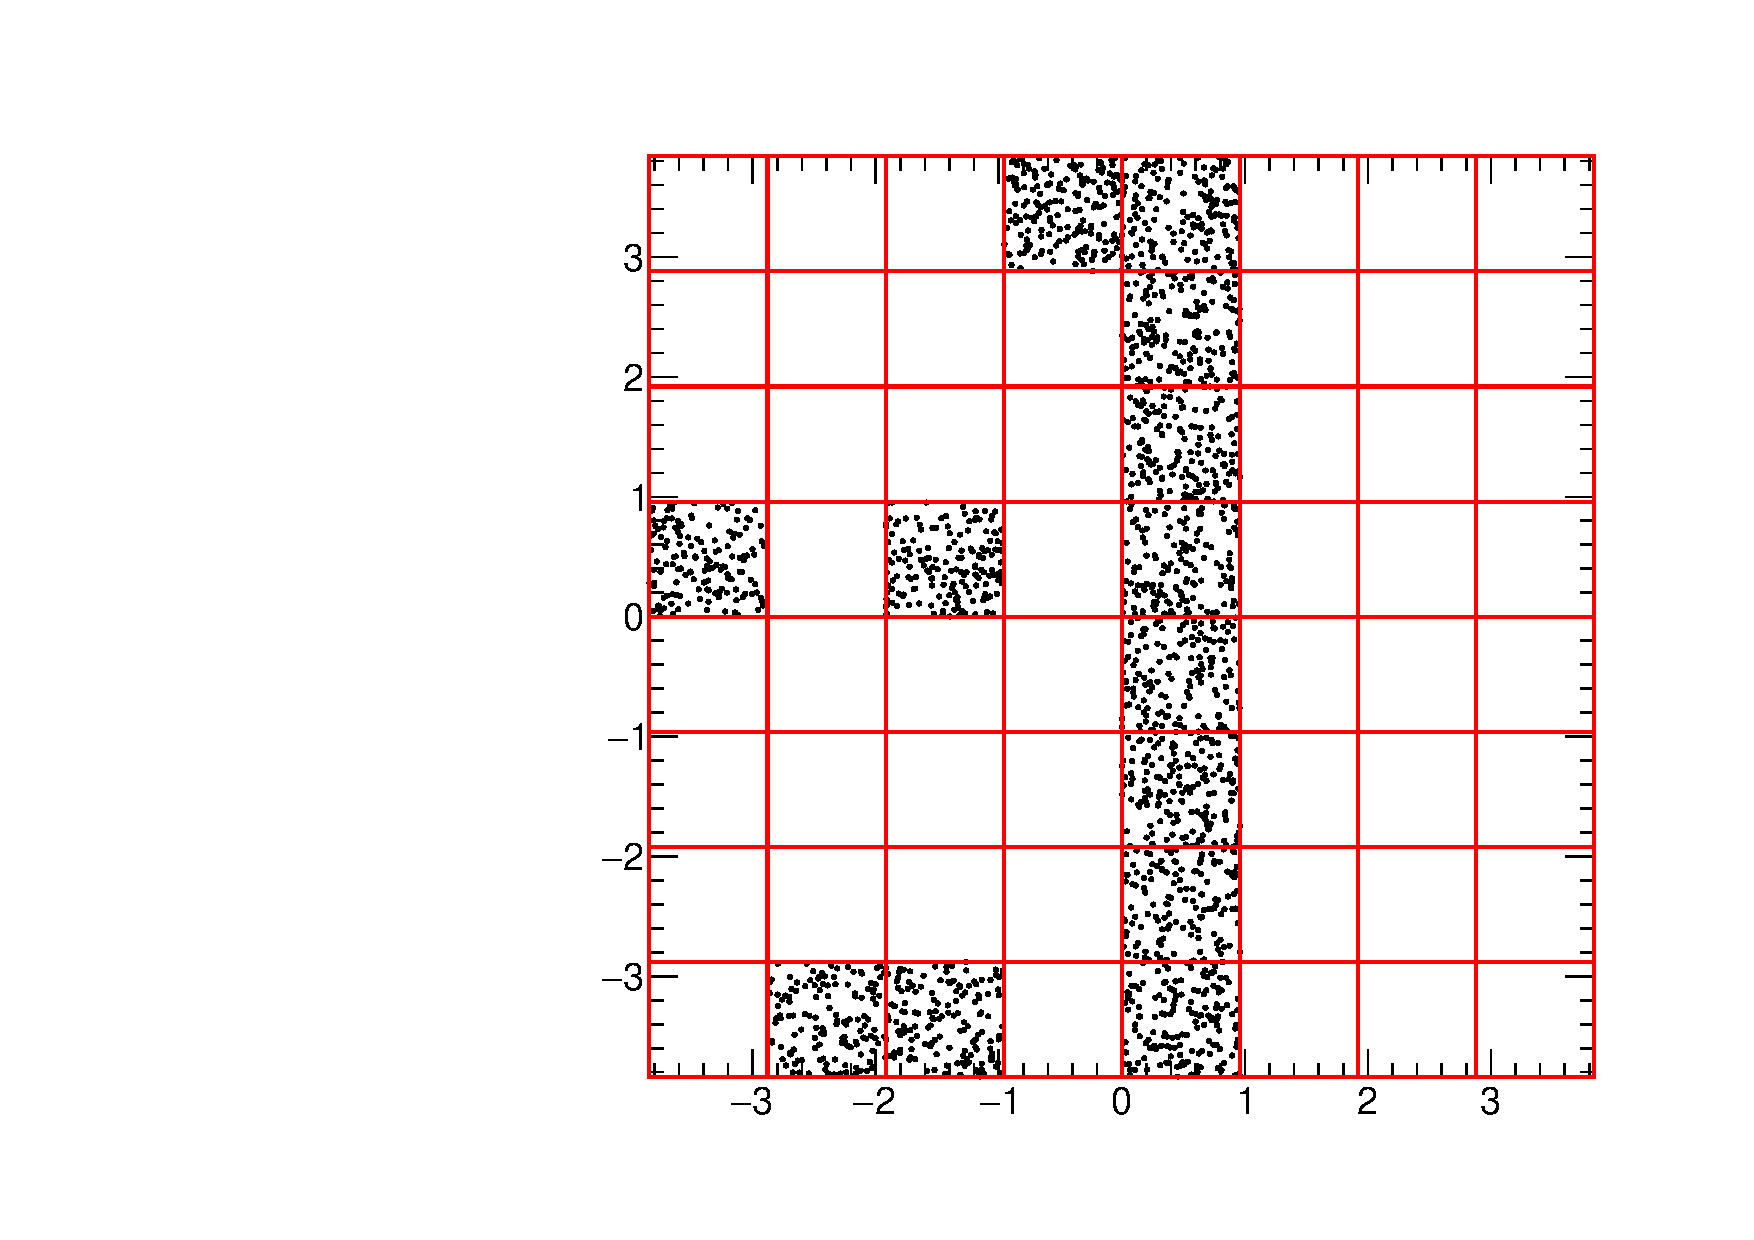
\includegraphics[width=0.3\linewidth]{images/pixel.pdf}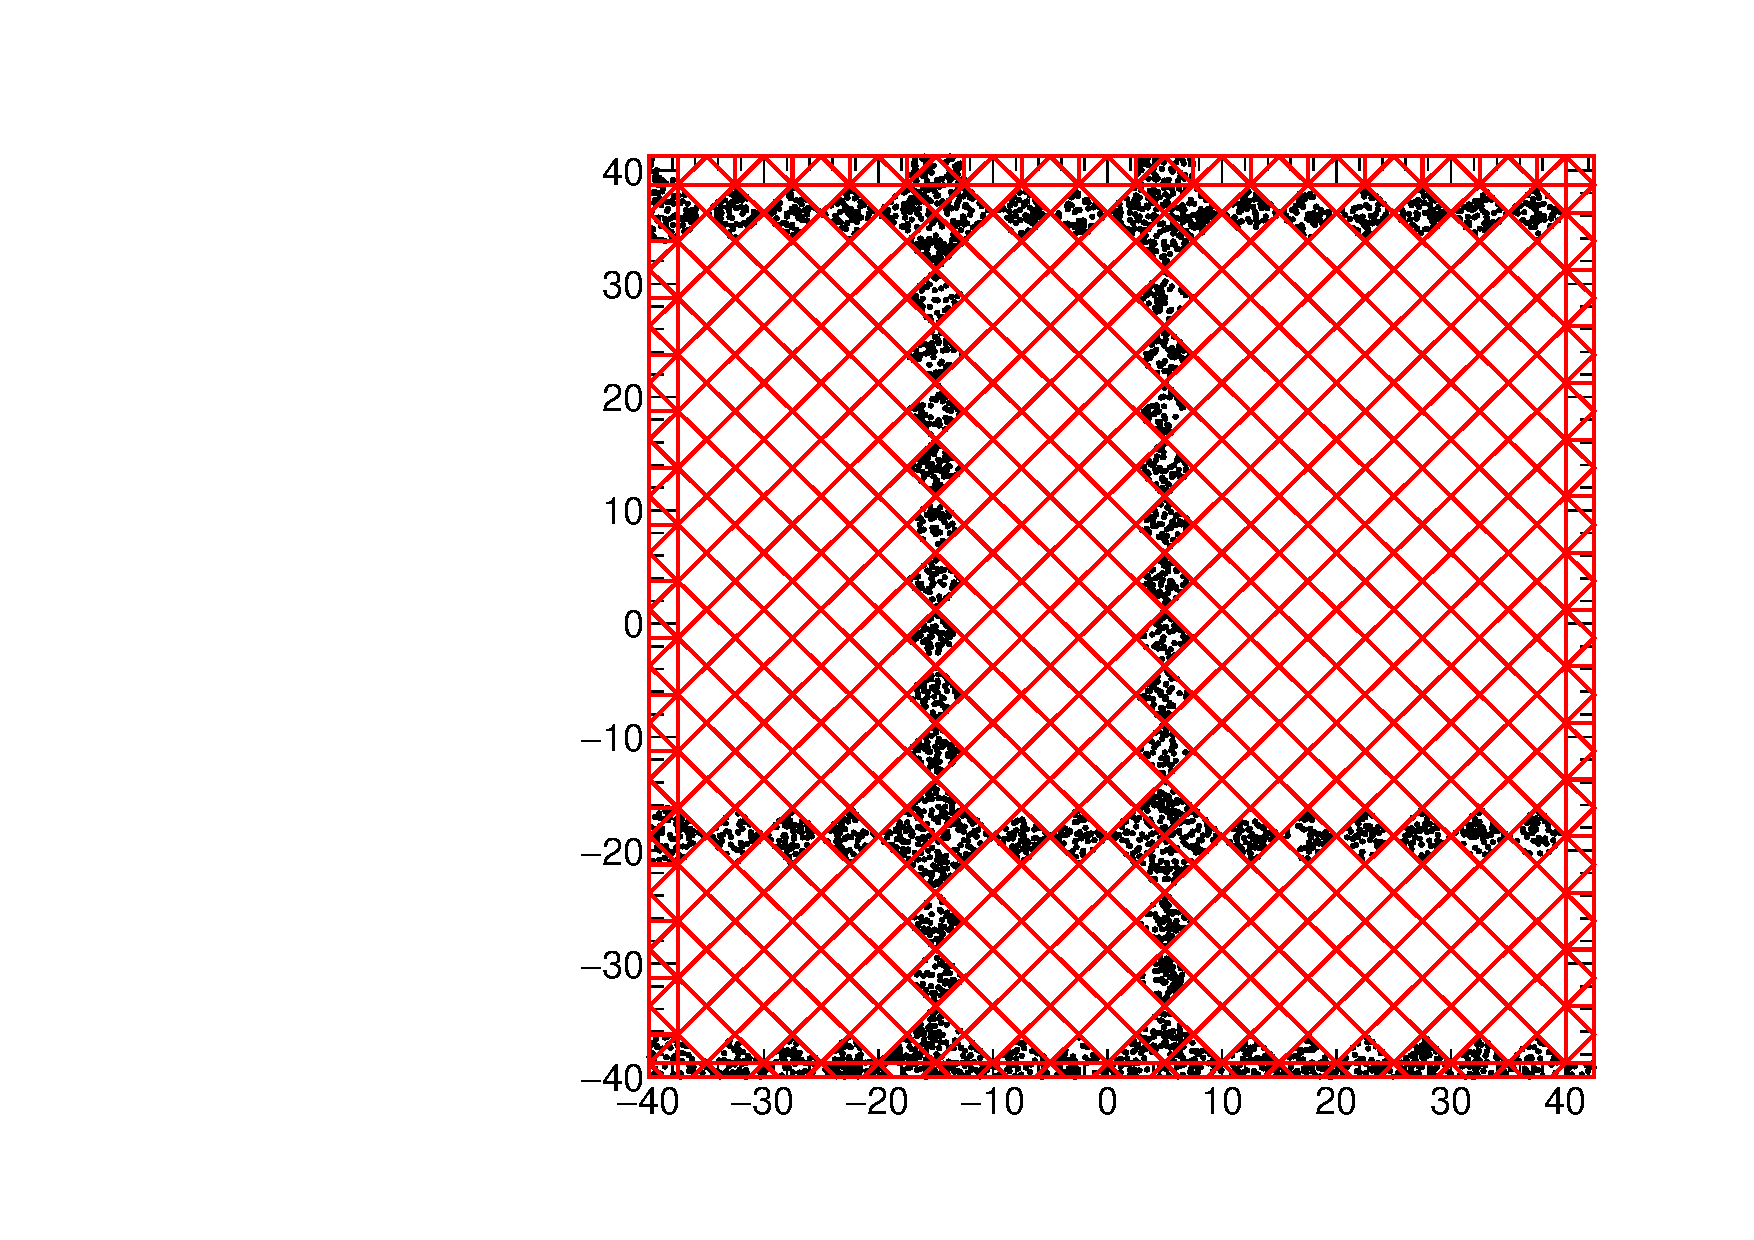
\includegraphics[width=0.3\linewidth]{images/microbulk.pdf}}
	\caption{}\label{fig:readouts}
\end{figure}

\subsection{The raw library}

The raw library\footnote{\url{https://github.com/rest-for-physics/rawlib}} is used to store time event pulses with a fixed number of bins. It includes processes related to signal conditioning, such as signal shaping, deconvolution, pulse fitting, de-noising, FFT, common noise reduction, and related routines. It is capable to read different binary formats from different electronic systems into REST.

\begin{figure}[hb!]
  \centering
  \raisebox{-0.5\height}{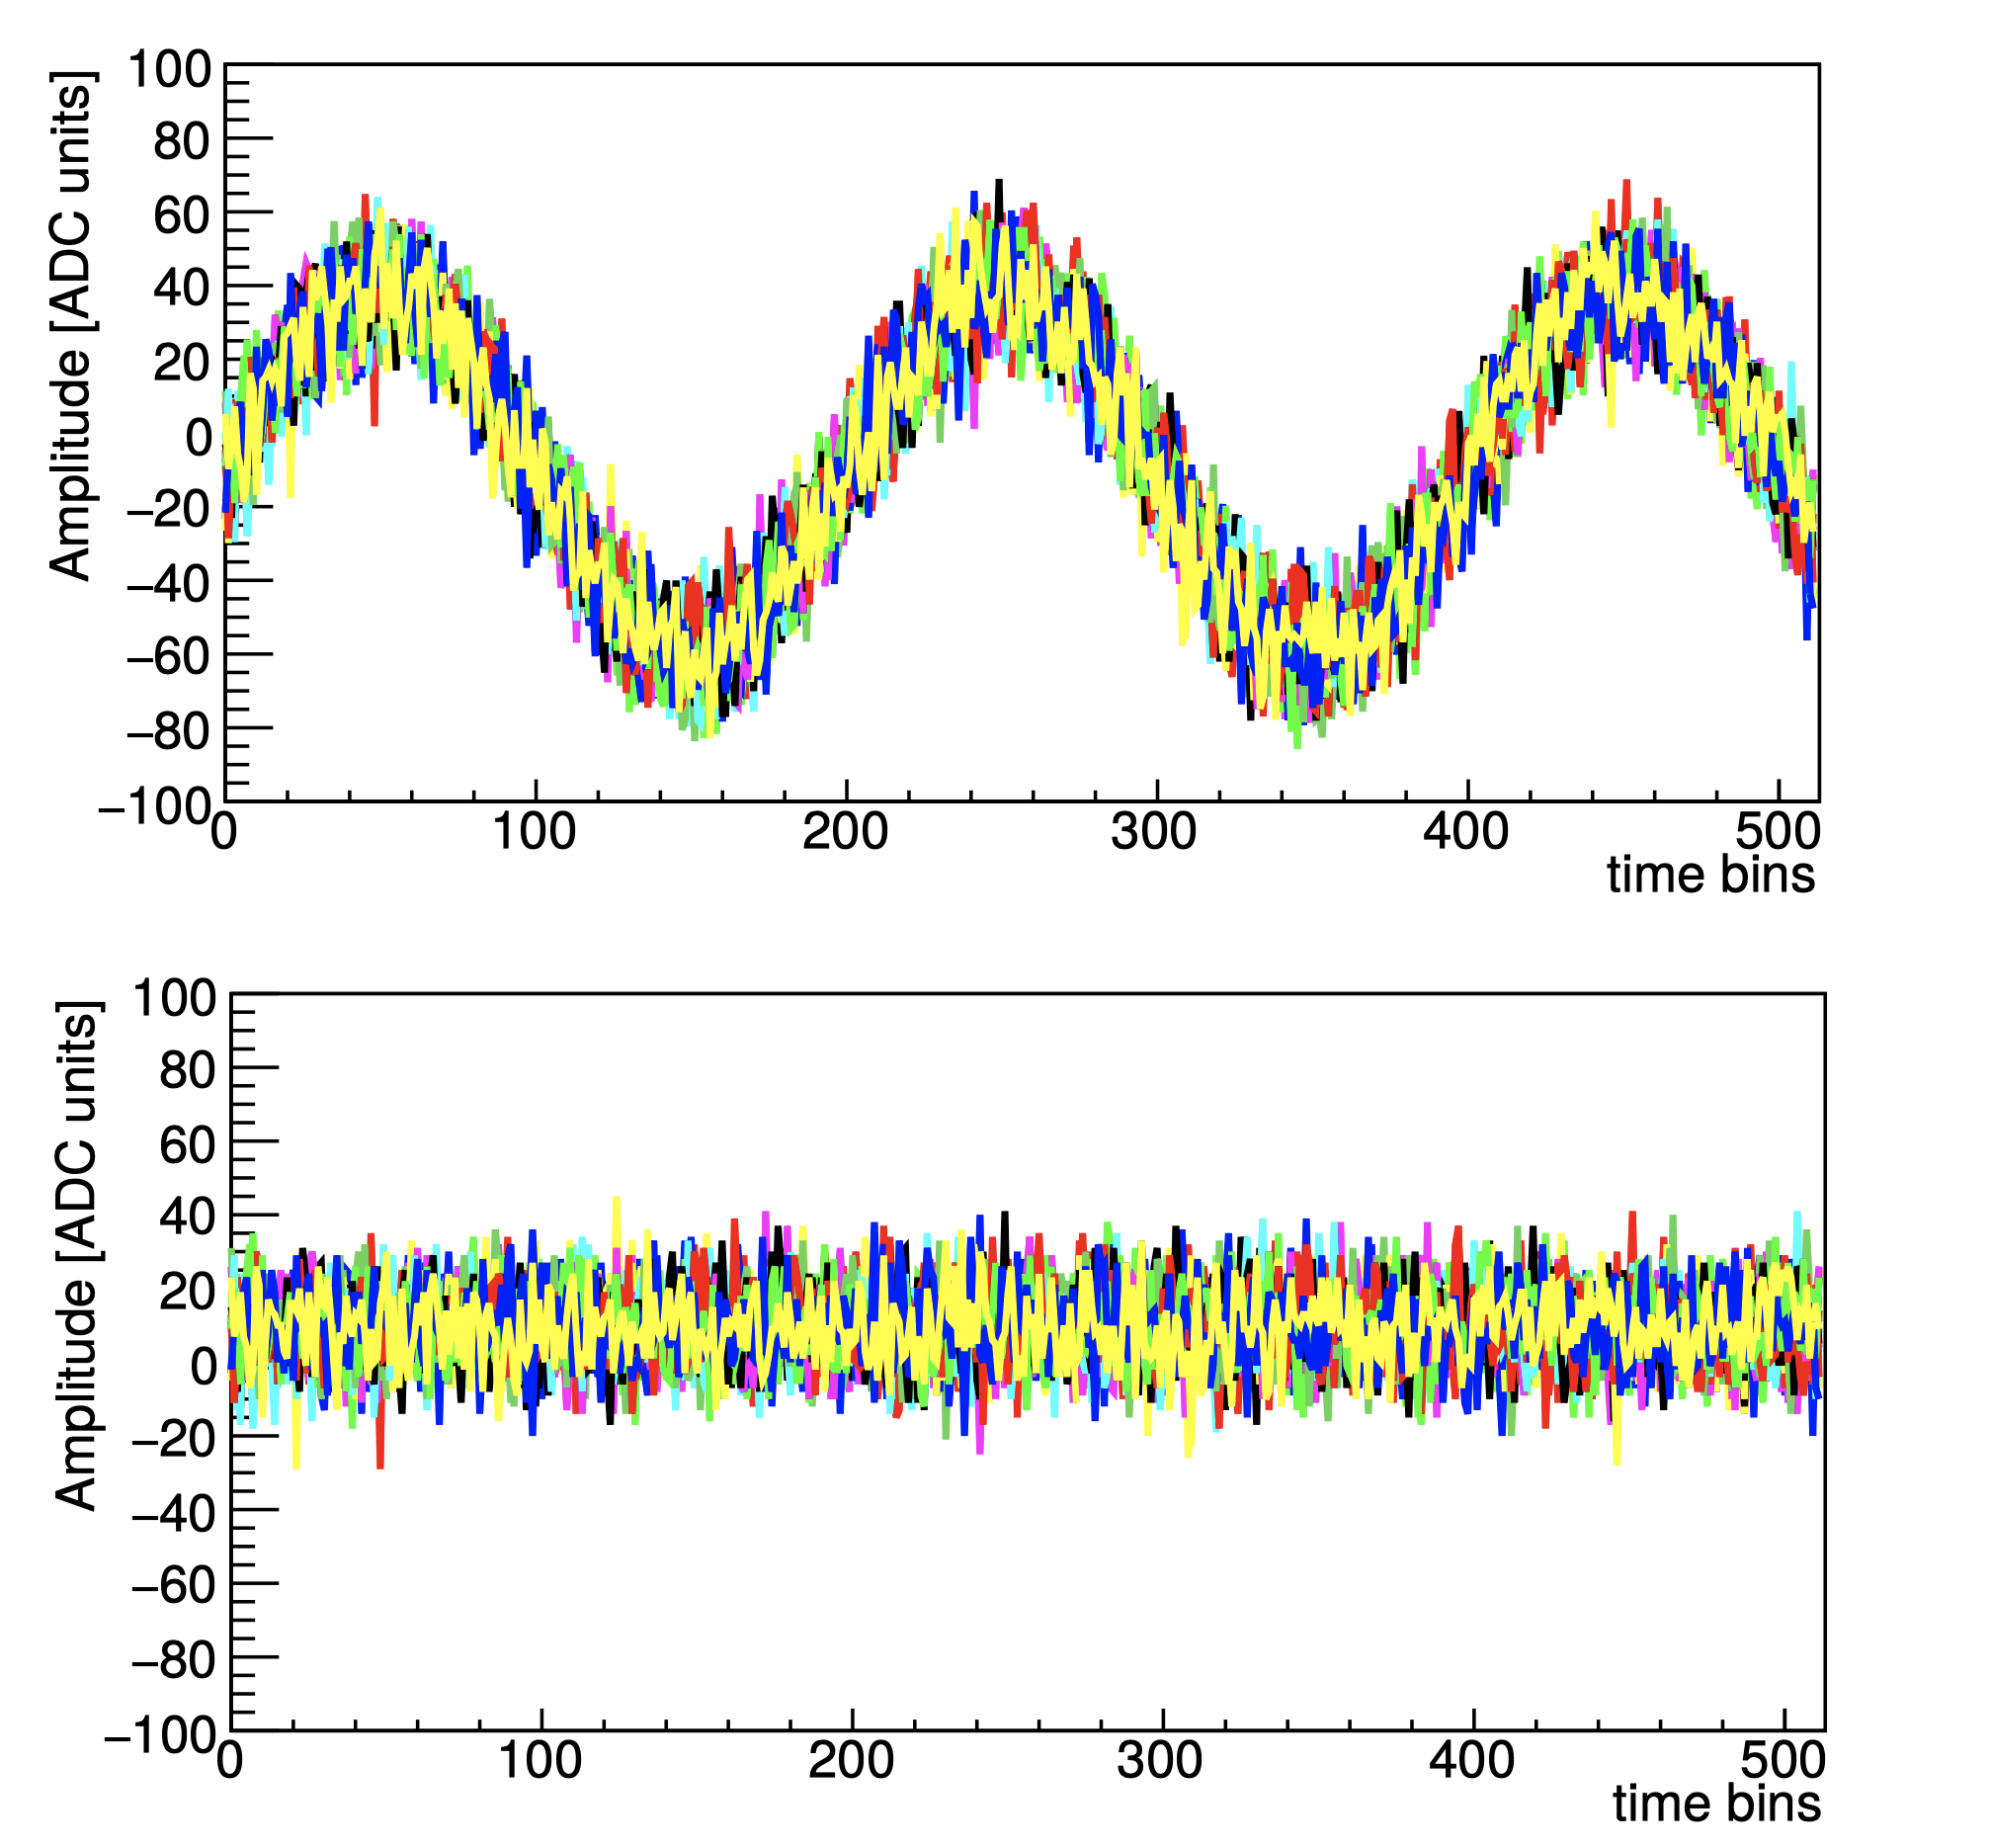
\includegraphics[totalheight=4cm]{images/commonNoise.png}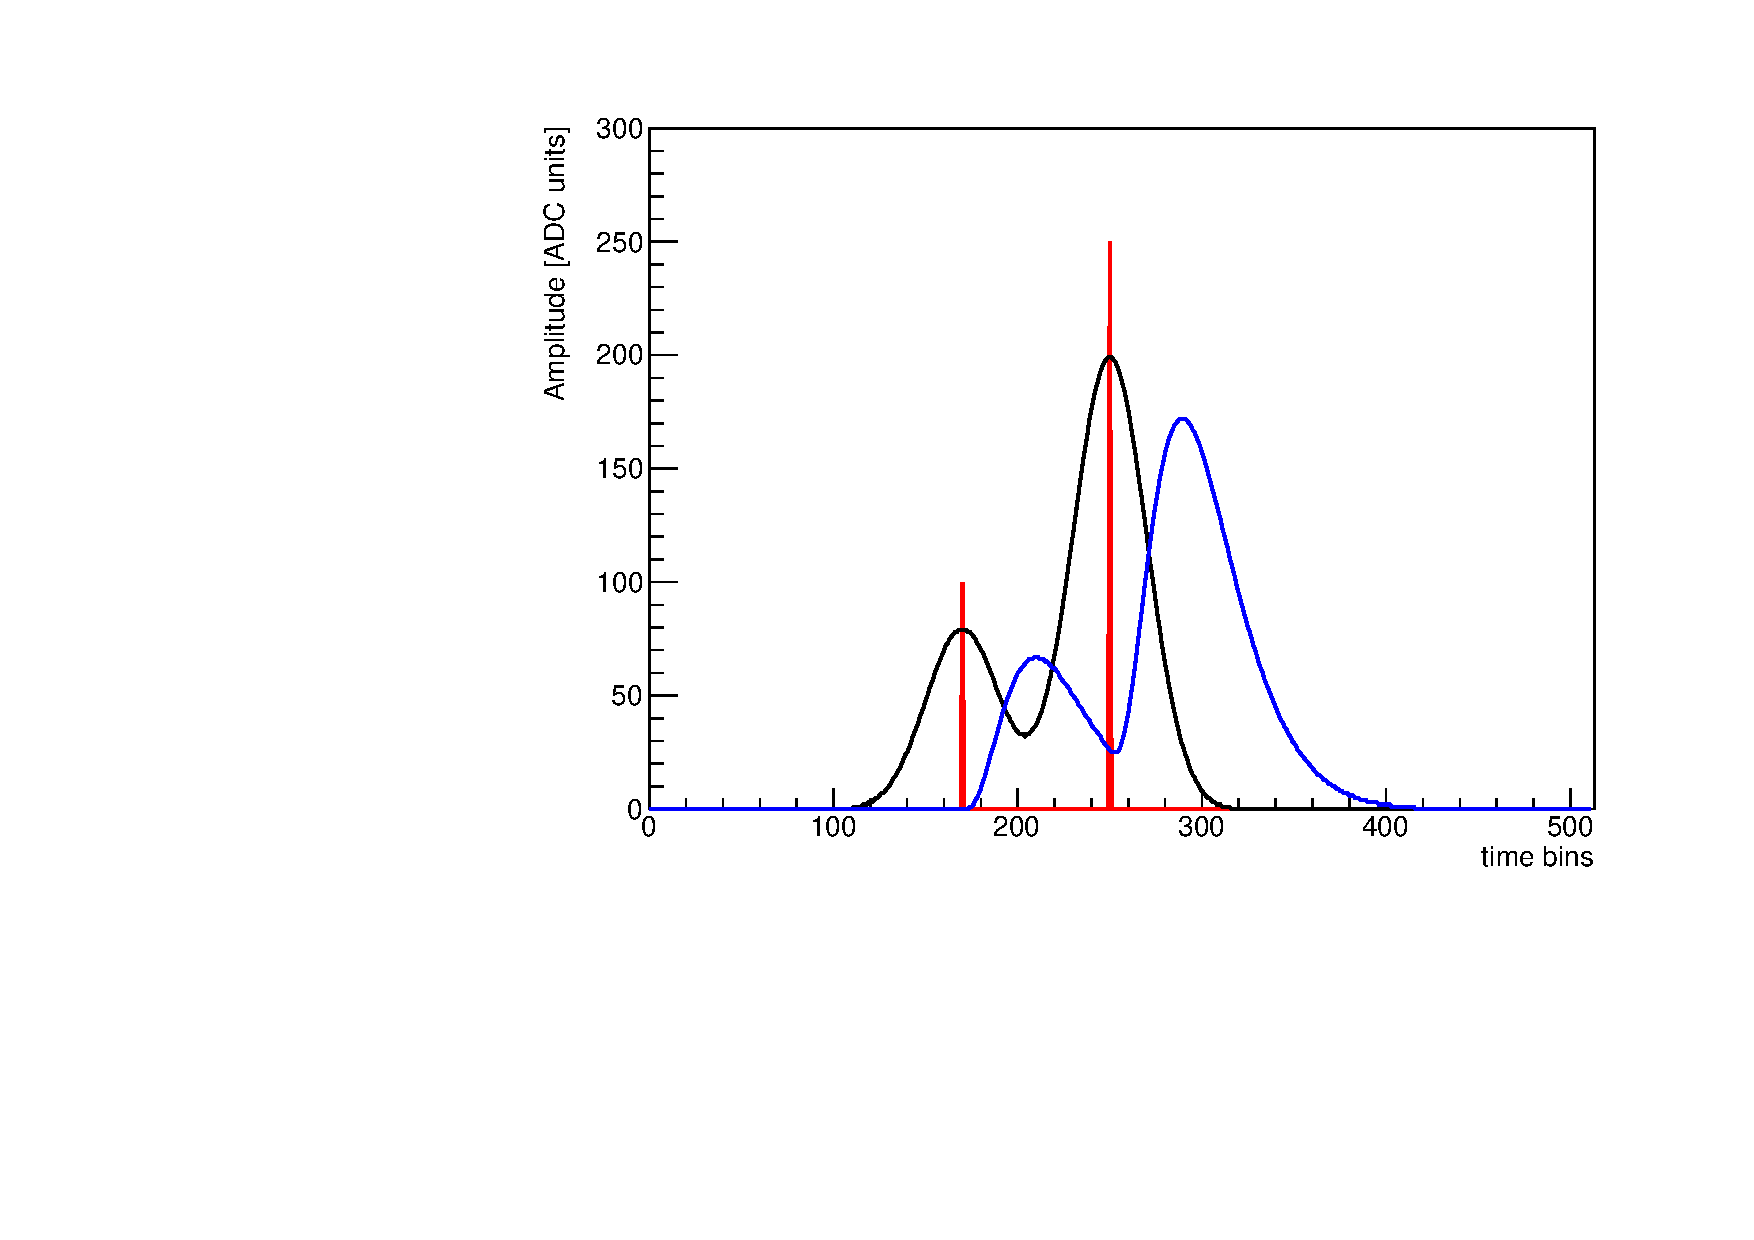
\includegraphics[totalheight=4cm]{images/shapingPlot.pdf}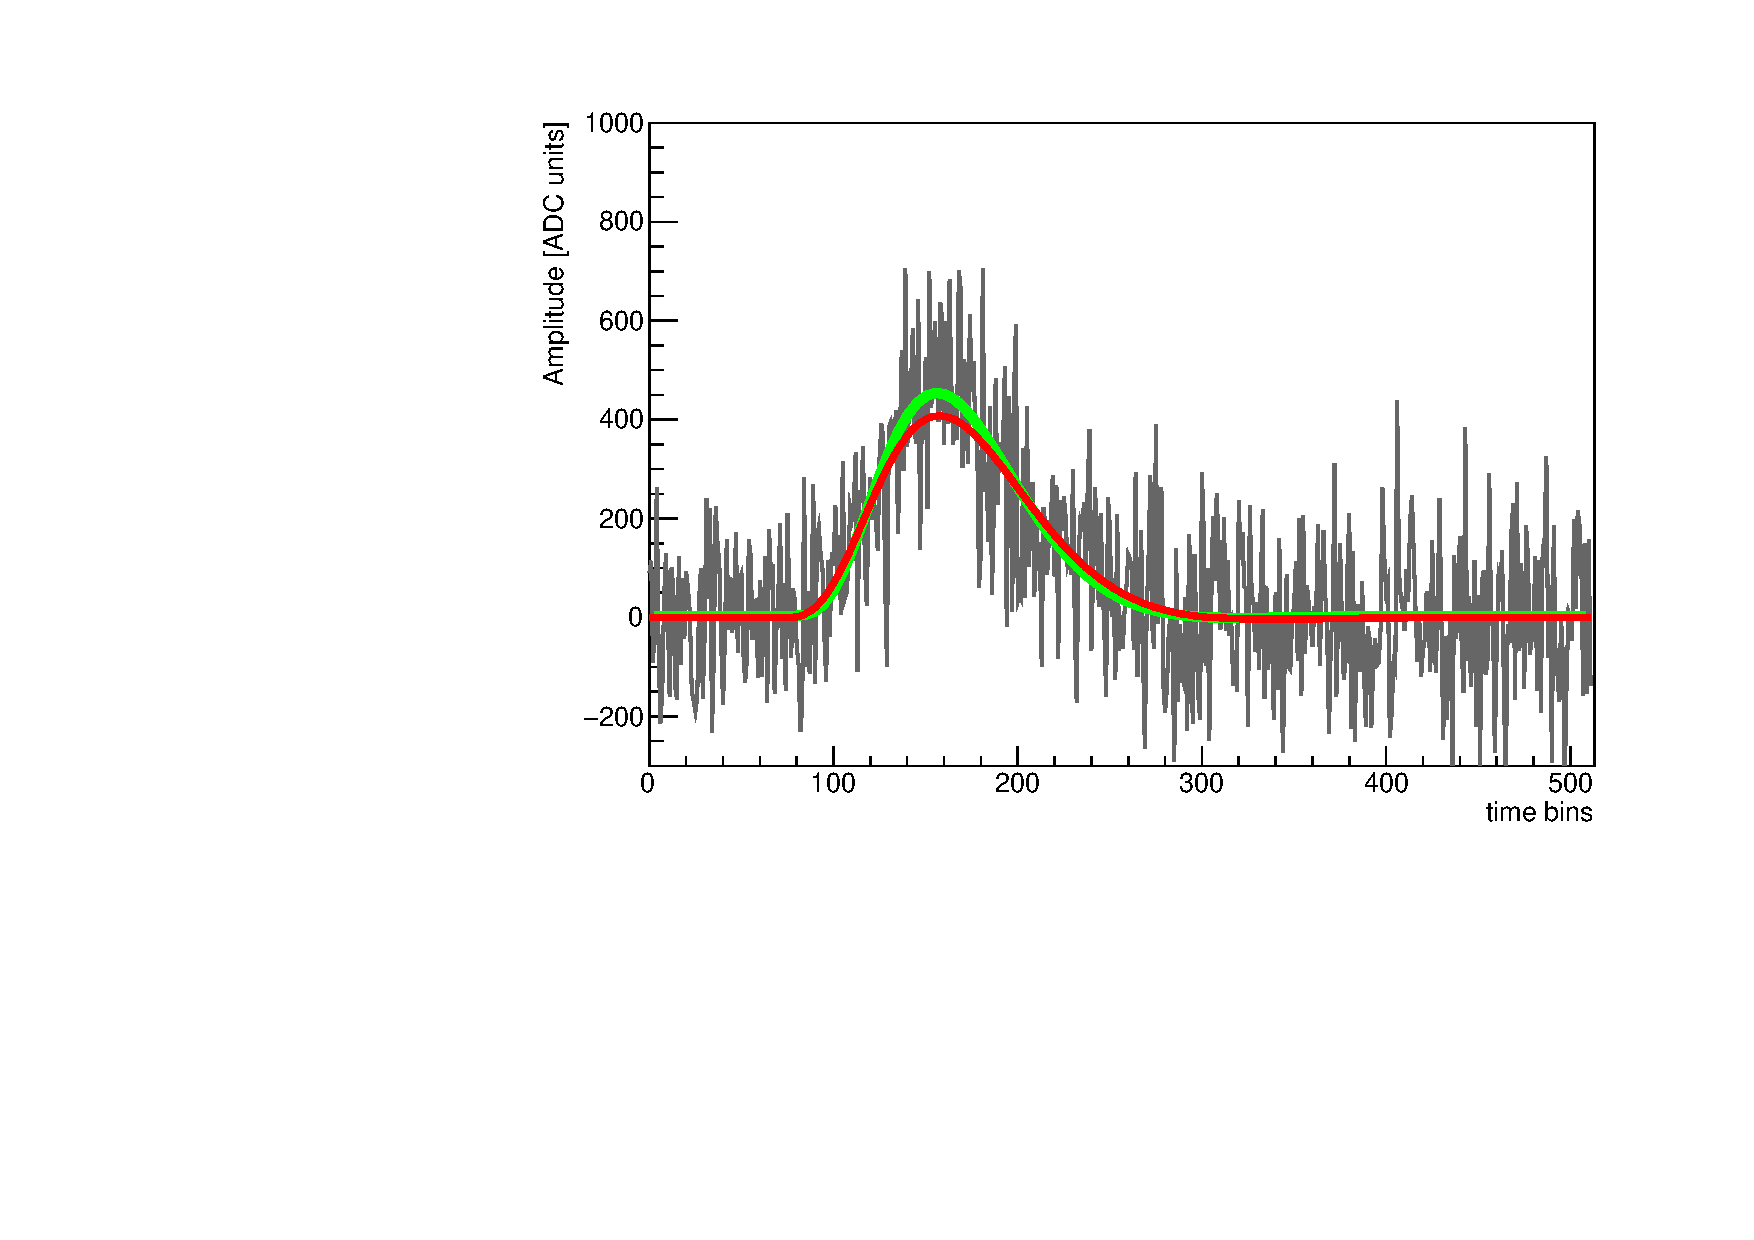
\includegraphics[totalheight=4cm]{images/fitComparison.pdf}}
	\caption{XX}\label{fig:rawlib}
\end{figure}

\subsection{The geant4 library}
the geant4 library\footnote{\url{https://github.com/rest-for-physics/geant4lib}} is used to store and analyse the events generated in a Geant4 simulation, it defines and stores the particle generator and simulation conditions, such as the details of the physics list used during the Monte Carlo.

\subsection{The track library}

The track library\footnote{\url{https://github.com/rest-for-physics/tracklib}} defines a track event type allowing to define inheritance relations between tracks that contain groups of hits. A process connecting to the detector library allows for hit clustering to create a first set of tracks using a distance relation. Graph theory processes are included in this library in order to identify and reconstruct a physical track, and execute topological algorithms.

\begin{figure}
\centering
    \raisebox{-0.5\height}{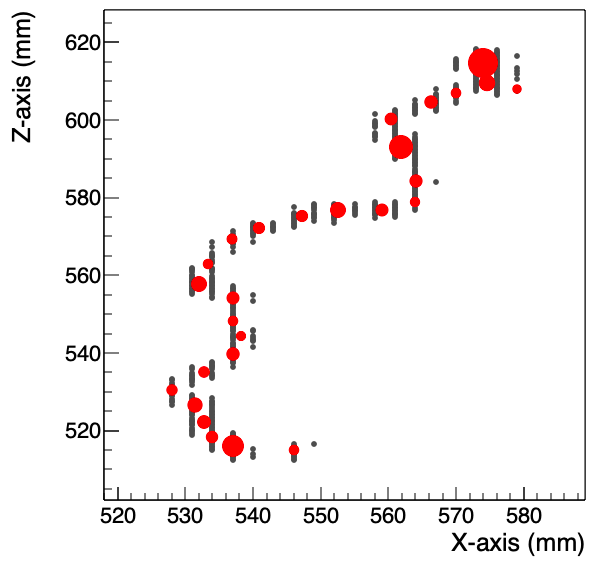
\includegraphics[totalheight=4.9cm]{images/TrackReduction.png}
    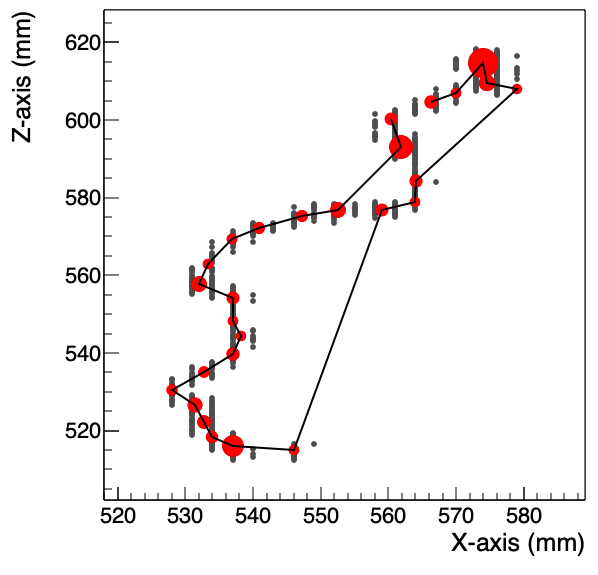
\includegraphics[totalheight=4.9cm]{images/TrackMinimized.png}
    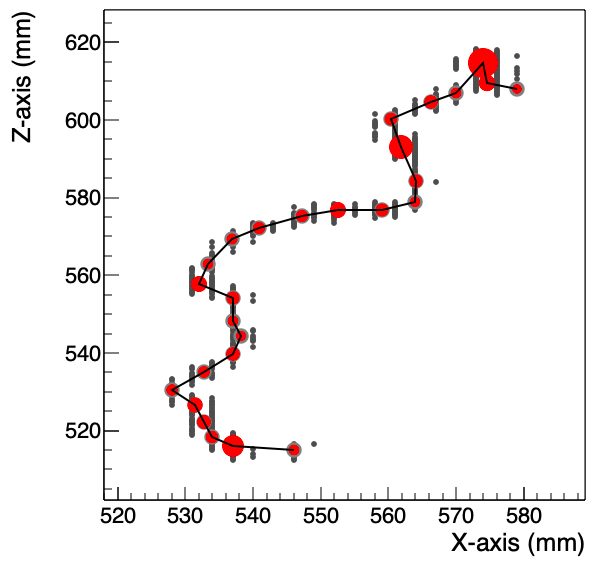
\includegraphics[totalheight=4.9cm]{images/TrackReconnected.png}}
    \caption{xxx}
    \label{fig:tracklib}
\end{figure}

\subsection{The connectors library}

The connectors library\footnote{\url{https://github.com/rest-for-physics/connectorslib}} contains different processes that inter-connect fundamental REST libraries, requiring to transfer an event type into another. I.e. hit clustering to transform detector hits into a track event, or raw signal to be transformed into a detector event. It also may contain other complex processes that require to use 2 libraries simultaneously.

\begin{figure}[hb!]
  \centering
  \raisebox{-0.5\height}{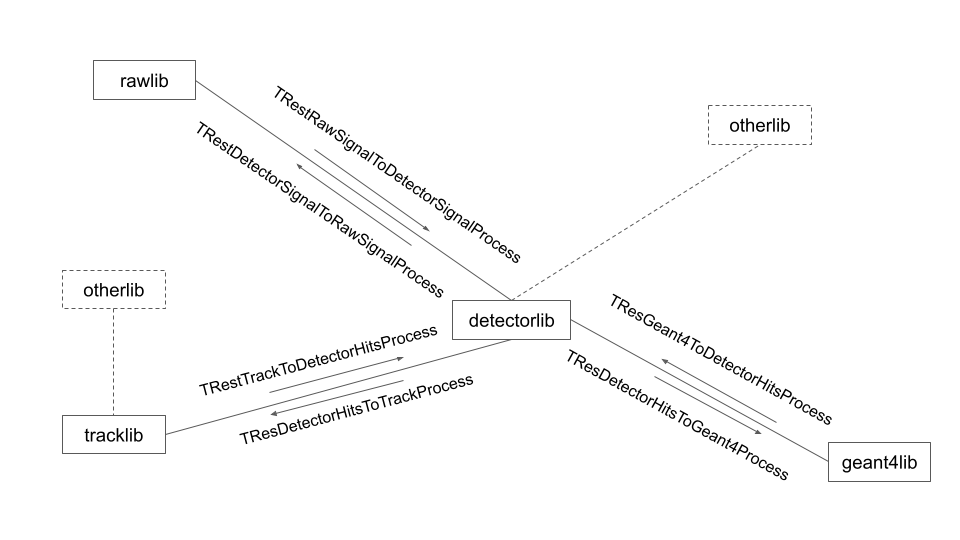
\includegraphics[width=0.75\linewidth]{images/connectorslib.png}}
	\caption{}\label{fig:connectorslib}
\end{figure}






\section{Summary}


%We are not presenting new technology or advanced bla bla bla, we are putting together the tools we use to process and analyse data in our physics domain context. Giving it robustness, bla bla bla

%We use ROOT to avoid worrying about I/O serialization and to find a solution bla bla bla, large community, long term support, etc.

%Future RDataFrame
\acknowledgments
We acknowledge support from the the European Research Council (ERC) under the European Union’s Horizon 2020 research and innovation programme, grant agreement ERC-2017-AdG788781 (IAXO+), and from the Spanish Agencia Estatal de Investigacion under grant FPA2016-76978-C3-1-P.

%\begin{figure}[htb!]
  \centering
  \raisebox{-0.5\height}{
\includegraphics[width=0.99\linewidth]{images/institution_logos.png}}
%\end{figure}

%\section*{References}
\bibliography{paper}
\bibliographystyle{unsrt}

% We suggest to always provide author, title and journal data:
% in short all the informations that clearly identify a document.

%\begin{thebibliography}{99}

%\bibitem{a}
%Author, \emph{Title}, \emph{J. Abbrev.} {\bf vol} (year) pg.

%\bibitem{b}
%Author, \emph{Title},
%arxiv:1234.5678.

%\bibitem{c}
%Author, \emph{Title},
%Publisher (year).


% Please avoid comments such as "For a review'', "For some examples",
% "and references therein" or move them in the text. In general,
% please leave only references in the bibliography and move all
% accessory text in footnotes.

% Also, please have only one work for each \bibitem.



\end{document}